%iffalse
\let\negmedspace\undefined
\let\negthickspace\undefined
\documentclass[journal,12pt,onecolumn]{IEEEtran}
\usepackage{cite}
\usepackage{amsmath,amssymb,amsfonts,amsthm}
\usepackage{algorithmic}
\usepackage{graphicx}
\usepackage{textcomp}
\usepackage{xcolor}
\usepackage{txfonts}
\usepackage{listings}
\usepackage{enumitem}
\usepackage{enumitem,multicol}
\usepackage{mathtools}
\usepackage{gensymb}
\usepackage{comment}
\usepackage[breaklinks=true]{hyperref}
\usepackage{tkz-euclide} 
\usepackage{listings}
\usepackage{gvv}                                        
%\def\inputGnumericTable{}                                 
\usepackage[latin1]{inputenc}                                
\usepackage{color}                                            
\usepackage{array}                                            
\usepackage{longtable}                                       
\usepackage{calc}                                             
\usepackage{multirow}                                         
\usepackage{hhline}                                           
\usepackage{ifthen}                                           
\usepackage{lscape}
\usepackage{tabularx}
\usepackage{array}
\usepackage{float}
\usepackage[american,siunitx]{circuitikz}
\usetikzlibrary{arrows,shapes,calc,positioning}
\usepackage{pgfplots}


\newtheorem{theorem}{Theorem}[section]
\newtheorem{problem}{Problem}
\newtheorem{proposition}{Proposition}[section]
\newtheorem{lemma}{Lemma}[section]
\newtheorem{corollary}[theorem]{Corollary}
\newtheorem{example}{Example}[section]
\newtheorem{definition}[problem]{Definition}
\newcommand{\BEQA}{\begin{eqnarray}}
\newcommand{\EEQA}{\end{eqnarray}}
\newcommand{\define}{\stackrel{\triangle}{=}}
\theoremstyle{remark}
\newtheorem{rem}{Remark}
\pgfplotsset{compat=1.18}

% Marks the beginning of the document
\begin{document}
\bibliographystyle{IEEEtran}
\vspace{3cm}

\title{EE-2023}
\author{EE24Btech11022 - Eshan Sharma}
\maketitle

\renewcommand{\thefigure}{\theenumi}
\renewcommand{\thetable}{\theenumi}



\begin{enumerate}
\item Which of the following statement(s) is/are true?

\begin{enumerate}
	\item If an LTI system is causal, it is stable.
	\item A discrete time LTI system is causal if and only if its response to a step input $u[n]$ is $0$ for $n < 0$.
	\item If a discrete time LTI system has an impulse response $h[n]$ of finite duration, the system is stable.
	\item If the impulse response $0 < |h[n]| < 1$ for all $n$, then the LTI system is stable.
\end{enumerate}

\item The bus admittance ($Y_{\text{bus}}$) matrix of a 3-bus power system is given below.
\[
Y_{\text{bus}} = 
\begin{bmatrix}
	-j15 & j10 & j5 \\
	j10 & -j13.5 & j4 \\
	j5 & j4 & -j8
\end{bmatrix}
\]
Considering that there is no shunt inductor connected to any of the buses, which of the following can NOT be true?

\begin{enumerate}
	\item Line charging capacitor of finite value is present in all three lines
	\item Line charging capacitor of finite value is present in line 2-3 only
	\item Line charging capacitor of finite value is present in line 2-3 only and shunt capacitor of finite value is present in bus 1 only
	\item Line charging capacitor of finite value is present in line 2-3 only and shunt capacitor of finite value is present in bus 3 only
\end{enumerate}

\item The value of parameters of the circuit shown in the figure are:\\
\begin{center}
$
R_1 = 2 \, \Omega, \quad R_2 = 2 \, \Omega, \quad R_3 = 3 \, \Omega, \quad L = 10 \, \text{mH}, \quad C = 100 \, \mu\text{F}
$
\end{center}
For time $t < 0$, the circuit is at steady state with the switch 'K'  in closed condition. If the switch is opened at $t = 0$, the value of the voltage across the inductor ($V_L$) at $t = 0^+$ in Volts is \_\_\_\_\_\_\_ (Round off to 1 decimal place).

\begin{center}
	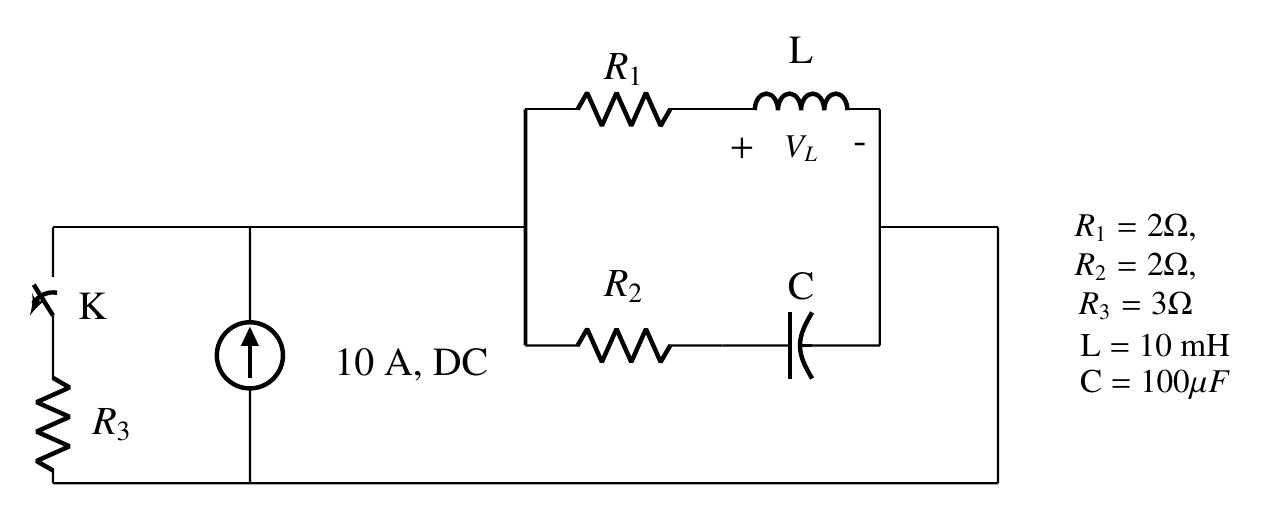
\begin{tikzpicture}[scale = 1]
		\tikzstyle{every node}=[font=\LARGE]
		\draw [ line width=1.4pt](12.25,15.25) to[short] (12.25,12.25);
		\draw [ line width=0.8](8.75,10.5) to[american current source] (8.75,13.75);
		\draw [line width=0.8pt](6.25,12) to[opening switch] (6.25,13.75);
		\draw [ line width=0.8pt](6.25,12) to[R] (6.25,10.5);
		\draw [ line width=0.8pt](6.25,13.75) to[short] (12.25,13.75);
		\draw [ line width=0.8pt](12.25,15.25) to[R] (14.75,15.25);
		\draw [ line width=0.8pt](12.25,12.25) to[R] (14.75,12.25);
		\draw [line width=0.8pt](14.75,15.25) to[L ] (16.75,15.25);
		\draw [line width=0.8pt](14.75,12.25) to[curved capacitor] (16.75,12.25);
		\draw [ line width=0.8pt](16.75,15.25) to[short] (16.75,12.25);
		\draw [ line width=0.8pt](16.75,13.75) to[short] (18.25,13.75);
		\draw [ line width=0.8pt](18.25,13.75) to[short] (18.25,10.5);
		\draw [ line width=0.8pt](6.25,10.5) to[short] (18.25,10.5);
		\node [font=\Large] at (15,14.75) {+};
		\node [font=\Large] at (16.5,14.75) {-};
		\node [font=\Large] at (10.8,12) {10 A, DC};
		\node [font=\Large] at (6.75,12.75) {K};
		\node [font=\Large] at (7,11.25) {$R_3$};
		\node [font=\Large] at (13.5,15.75) {$R_1$};
		\node [font=\Large] at (13.5,13) {$R_2$};
		\node [font=\Large] at (15.75,13) {C};
		\node [font=\Large] at (15.75,16) {L};
		\node [font=\large] at (15.75,14.75) {$V_L$};
		\node [font=\large] at (20,13.75) {$R_1 = 2\Omega$,};
		\node [font=\large] at (20,13.25) {$R_2 = 2\Omega$,};
		\node [font=\large] at (20,12.75) {$R_3 = 3\Omega$};
		\node [font=\large] at (20.25,12.25) {L = 10 mH};
		\node [font=\large] at (20.25,11.75) {C = 100$\mu F$};
	\end{tikzpicture}
\end{center}

\item A separately excited DC motor rated $400 \, \text{V}$, $15 \, \text{A}$, $1500 \, \text{RPM}$ drives a constant torque load at rated speed operating from $400 \, \text{V}$ DC supply drawing rated current. The armature resistance is $1.2 \, \Omega$. If the supply voltage drops by $10\%$ with field current unaltered, then the resultant speed of the motor in RPM is $\_\_\_\_\_\_\_$ (Round off to the nearest integer).\\
	
\item For the signals $x(t)$ and $y(t)$ shown in the figure, $z(t) = x(t) * y(t)$ is maximum at $t = T_1$. Then $T_1$ in seconds is $\_\_\_\_\_\_\_$ (Round off to the nearest integer).\\

\begin{center}
	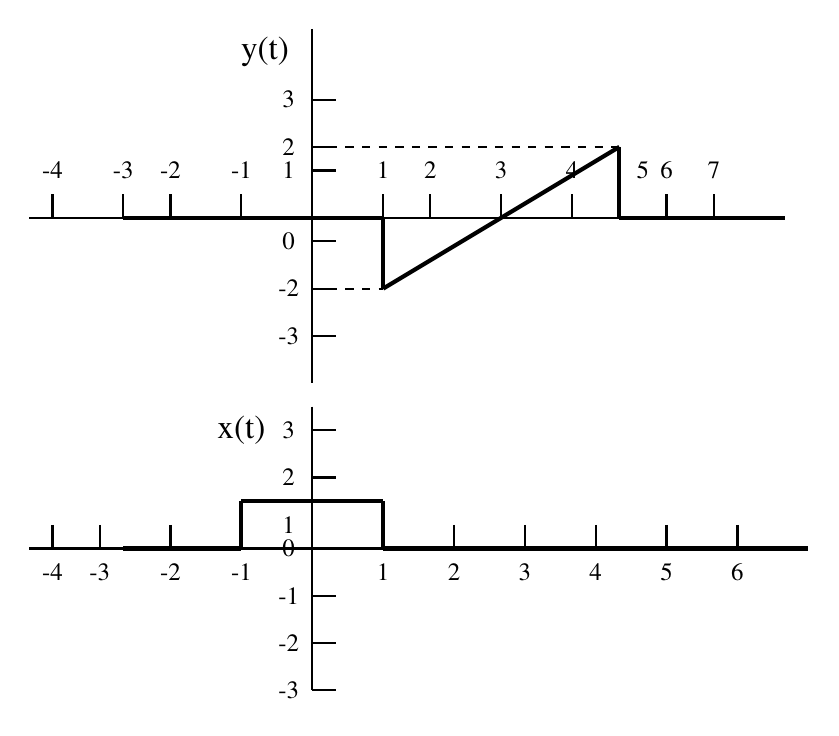
\begin{tikzpicture}[scale = 1.2]
		\tikzstyle{every node}=[font=\small]
		\draw [line width=0.8pt, short] (5.5,13.5) -- (12.5,13.5);
		\draw [line width=0.8pt, short] (7.5,15.5) -- (7.5,11.75);
		\draw [line width=0.8pt, short] (7.5,11.5) -- (7.5,8.5);
		\draw [line width=0.8pt, short] (5.5,10) -- (12.75,10);
		\draw [line width=1.5pt, short] (5.5,13.5) -- (8.25,13.5);
		\draw [line width=1.5pt, short] (8.25,13.5) -- (8.25,12.75);
		\draw [line width=1.5pt, short] (8.25,12.75) -- (10.75,14.25);
		\draw [line width=1.5pt, short] (10.75,14.25) -- (10.75,13.5);
		\draw [line width=1.5pt, short] (10.75,13.5) -- (12.5,13.5);
		\draw [line width=1.5pt, short] (5.5,10) -- (6.75,10);
		\draw [line width=1.5pt, short] (6.75,10) -- (6.75,10.5);
		\draw [line width=1.5pt, short] (6.75,10.5) -- (8.25,10.5);
		\draw [line width=1.5pt, short] (8.25,10.5) -- (8.25,10);
		\draw [line width=1.5pt, short] (8.25,10) -- (12.75,10);
		\draw [line width=0.8pt, short] (5.5,13.5) -- (4.5,13.5);
		\draw [line width=0.8pt, short] (5.5,10) -- (4.5,10);
		\draw [line width=0.8pt, dashed] (7.5,14.25) -- (10.75,14.25);
		\draw [line width=0.8pt, dashed] (7.5,12.75) -- (8.25,12.75);
		\node [font=\large] at (7,15.25) {y(t)};
		\node [font=\large] at (6.75,11.25) {x(t)};
		\draw [line width=0.8pt, short] (7.5,14) -- (7.75,14);
		\draw [line width=0.8pt, short] (7.5,14.25) -- (7.75,14.25);
		\draw [line width=0.8pt, short] (7.5,14.75) -- (7.75,14.75);
		\draw [line width=0.8pt, short] (7.5,13.25) -- (7.75,13.25);
		\draw [line width=0.8pt, short] (7.5,12.75) -- (7.75,12.75);
		\draw [line width=0.8pt, short] (7.5,12.25) -- (7.75,12.25);
		\draw [line width=0.8pt, short] (8.25,13.75) -- (8.25,13.5);
		\draw [line width=0.8pt, short] (8.75,13.75) -- (8.75,13.5);
		\draw [line width=0.8pt, short] (9.5,13.75) -- (9.5,13.5);
		\draw [line width=0.8pt, short] (10.25,13.75) -- (10.25,13.5);
		\draw [line width=0.8pt, short] (10.75,13.75) -- (10.75,13.5);
		\draw [line width=0.8pt, short] (11.25,13.75) -- (11.25,13.5);
		\draw [line width=0.8pt, short] (11.75,13.75) -- (11.75,13.5);
		\draw [line width=0.8pt, short] (6.75,13.75) -- (6.75,13.5);
		\draw [line width=0.8pt, short] (6,13.75) -- (6,13.5);
		\draw [line width=0.8pt, short] (5.5,13.75) -- (5.5,13.5);
		\draw [line width=0.8pt, short] (4.75,13.75) -- (4.75,13.5);
		\draw [line width=0.8pt, short] (7.5,10.5) -- (7.75,10.5);
		\draw [line width=0.8pt, short] (7.5,10.75) -- (7.75,10.75);
		\draw [line width=0.8pt, short] (7.5,11.25) -- (7.75,11.25);
		\draw [line width=0.8pt, short] (7.5,10) -- (7.75,10);
		\draw [line width=0.8pt, short] (7.5,9.5) -- (7.75,9.5);
		\draw [line width=0.8pt, short] (7.5,9) -- (7.75,9);
		\draw [line width=0.8pt, short] (7.5,8.5) -- (7.75,8.5);
		\draw [line width=0.8pt, short] (6.75,10.25) -- (6.75,10);
		\draw [line width=0.8pt, short] (8.25,10.25) -- (8.25,10);
		\draw [line width=0.8pt, short] (9,10.25) -- (9,10);
		\draw [line width=0.8pt, short] (9.75,10.25) -- (9.75,10);
		\draw [line width=0.8pt, short] (10.5,10.25) -- (10.5,10);
		\draw [line width=0.8pt, short] (11.25,10.25) -- (11.25,10);
		\draw [line width=0.8pt, short] (12,10.25) -- (12,10);
		\draw [line width=0.8pt, short] (6,10.25) -- (6,10);
		\draw [line width=0.8pt, short] (5.25,10.25) -- (5.25,10);
		\draw [line width=0.8pt, short] (4.75,10.25) -- (4.75,10);
		\node [font=\small] at (7.25,13.25) {0};
		\node [font=\small] at (7.25,14) {1};
		\node [font=\small] at (7.25,14.25) {2};
		\node [font=\small] at (7.25,14.75) {3};
		\node [font=\small] at (8.25,14) {1};
		\node [font=\small] at (8.75,14) {2};
		\node [font=\small] at (9.5,14) {3};
		\node [font=\small] at (10.25,14) {4};
		\node [font=\small] at (11,14) {5};
		\node [font=\small] at (11.25,14) {6};
		\node [font=\small] at (11.75,14) {7};
		\node [font=\small] at (6.75,14) {-1};
		\node [font=\small] at (6,14) {-2};
		\node [font=\small] at (5.5,14) {-3};
		\node [font=\small] at (4.75,14) {-4};
		\node [font=\small] at (7.25,12.75) {-2};
		\node [font=\small] at (7.25,12.25) {-3};
		\node [font=\small] at (7.25,10.25) {1};
		\node [font=\small] at (7.25,10.75) {2};
		\node [font=\small] at (7.25,11.25) {3};
		\node [font=\small] at (7.25,10) {0};
		\node [font=\small] at (7.25,9.5) {-1};
		\node [font=\small] at (7.25,9) {-2};
		\node [font=\small] at (7.25,8.5) {-3};
		\node [font=\small] at (8.25,9.75) {1};
		\node [font=\small] at (9,9.75) {2};
		\node [font=\small] at (9.75,9.75) {3};
		\node [font=\small] at (10.5,9.75) {4};
		\node [font=\small] at (11.25,9.75) {5};
		\node [font=\small] at (12,9.75) {6};
		\node [font=\small] at (6.75,9.75) {-1};
		\node [font=\small] at (6,9.75) {-2};
		\node [font=\small] at (5.25,9.75) {-3};
		\node [font=\small] at (4.75,9.75) {-4};
	\end{tikzpicture}
\end{center}

\item For the circuit shown in the figure, $V_1 = 8$ V, DC and $I_1 = 8$ A, DC. The voltage $V_{ab}$ in Volts is $\_\_\_\_\_\_\_$ (Round off to 1 decimal place).\\

\begin{center}
	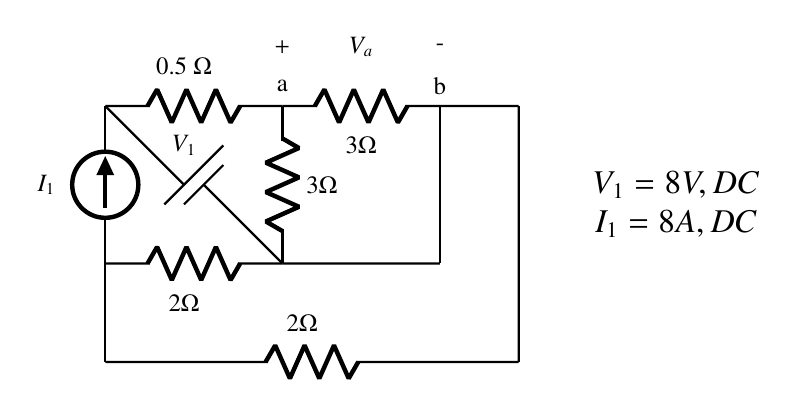
\begin{tikzpicture}[scale = 1]
		\tikzstyle{every node}=[font=\large]
		\draw [ line width=0.8pt](5.5,14.25) to[R] (7.75,14.25);
		\draw [ line width=0.8pt](7.75,14.25) to[R] (9.75,14.25);
		\draw [ line width=0.8pt](7.75,14.25) to[R] (7.75,12.25);
		\draw [ line width=0.8pt](5.5,12.25) to[R] (7.75,12.25);
		\draw [ line width=0.8pt](5.5,12.25) to[american current source] (5.5,14.25);
		\draw [ line width=0.8pt](7.75,12.25) to[short] (9.75,12.25);
		\draw [ line width=0.8pt](9.75,14.25) to[short] (9.75,12.25);
		\draw [ line width=0.8pt](9.75,14.25) to[short] (10.75,14.25);
		\draw [ line width=0.8pt](10.75,14.25) to[short] (10.75,11);
		\draw [ line width=0.8pt](5.5,12.25) to[short] (5.5,11);
		\draw [ line width=0.8pt](5.5,11) to[R] (10.75,11);
		\draw [line width=0.8pt, short] (5.5,14.25) -- (6.5,13.25);
		\draw [line width=0.8pt, short] (6.25,13) -- (7,13.75);
		\draw [line width=0.8pt, short] (6.5,13) -- (7,13.5);
		\draw [line width=0.8pt, short] (6.75,13.25) -- (7.75,12.25);
		\node [font=\small] at (4.75,13.25) {$I_1$};
		\node [font=\small] at (6.5,14.75) {0.5 $\Omega$};
		\node [font=\small] at (8.75,13.75) {3$\Omega$};
		\node [font=\small] at (8.25,13.25) {3$\Omega$};
		\node [font=\small] at (6.5,11.75) {2$\Omega$};
		\node [font=\small] at (8,11.5) {2$\Omega$};
		\node [font=\small] at (6.5,13.75) {$V_1$};
		\node [font=\small] at (7.75,14.5) {a};
		\node [font=\small] at (9.75,14.5) {b};
		\node [font=\small] at (7.75,15) {+};
		\node [font=\small] at (9.75,15) {-};
		\node [font=\small] at (8.75,15) {$V_a$};
		\node [font=\large] at (12.75,13.25) {$V_1 = 8V, DC$};
		\node [font=\large] at (12.75,12.75) {$I_1 = 8A,DC$};
	\end{tikzpicture}
\end{center}

\item A 50 Hz, 275 kV line of length 400 km has the following parameters: \\
Resistance, $R = 0.035 \, \Omega/\text{km}$; \\
Inductance, $L = 1 \, \text{mH} / \text{km}$; \\
Capacitance, $C = 0.01 \, \mu\text{F}/\text{km}$; \\
The line is represented by the nominal-$\pi$ model. With the magnitudes of the sending
end and the receiving end voltages of the line (denoted by $V_S$ and $V_R$, respectively)
maintained at 275 kV, the phase angle difference ($\theta$) between $V_S$ and $V_R$ required for
maximum possible active power to be delivered to the receiving end, in degrees is $\_\_\_\_\_\_\_$ (Round off to 2 decimal places).

\item In the following differential equation, the numerically obtained value of $y(t)$, at $t = 1$, is $\_\_\_\_\_\_\_$ (Round off to 2 decimal places).
\[
\frac{dy}{dt} = \frac{e^{-\alpha t}}{2 + \alpha t}, \quad \alpha = 0.01 \text{ and } y(0) = 0
\]

\item Three points in the $x$-$y$ plane are $(-1, 0.8)$, $(0, 2.2)$ and $(1, 2.8)$. The value of the slope of the best fit straight line in the least square sense is $\_\_\_\_\_\_\_$ (Round off to 2 decimal places).

\item The magnitude and phase plots of an LTI system are shown in the figure. The transfer function of the system is

\begin{center}
	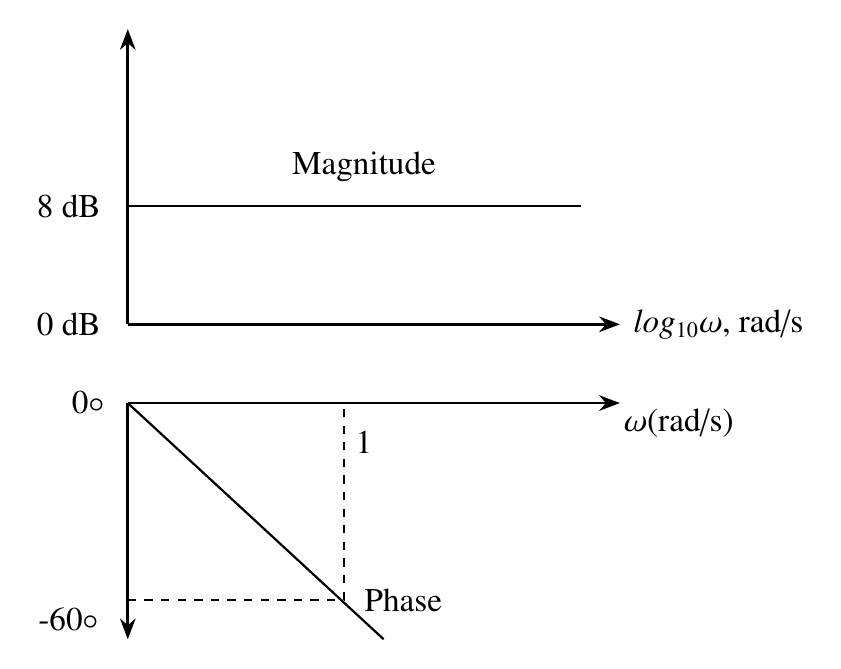
\begin{tikzpicture}[scale = 1]
		\tikzstyle{every node}=[font=\large]
		\draw [line width=1pt, ->, >=Stealth] (9.25,13.5) -- (9.25,17.25);
		\draw [line width=1pt, ->, >=Stealth] (9.25,13.5) -- (15.5,13.5);
		\draw [line width=1pt, ->, >=Stealth] (9.25,12.5) -- (15.5,12.5);
		\draw [line width=1pt, ->, >=Stealth] (9.25,12.5) -- (9.25,9.5);
		\draw [line width=0.8pt, short] (9.25,15) -- (15,15);
		\draw [line width=0.8pt, short] (9.25,12.5) -- (12.5,9.5);
		\draw [line width=0.8pt, dashed] (9.25,10) -- (12,10);
		\draw [line width=0.8pt, dashed] (12,10) -- (12,12.5);
		\node [font=\large] at (12.25,15.5) {Magnitude};
		\node [font=\large] at (12.75,10) {Phase};
		\node [font=\large] at (8.75,12.5) {0$\circ$};
		\node [font=\large] at (8.5,9.75) {-60$\circ$};
		\node [font=\large] at (12.25,12) {1};
		\node [font=\large] at (8.5,13.5) {0 dB};
		\node [font=\large] at (8.5,15) {8 dB};
		\node [font=\large] at (16.75,13.5) {$log_{10} \omega$, rad/s};
		\node [font=\large] at (16.25,12.25) {$\omega$(rad/s)};
	\end{tikzpicture}
\end{center}

\begin{enumerate}
	\item $2.51 e^{-0.032s}$
	\item $\frac{e^{-2.514s}}{s + 1}$
	\item $1.04 e^{-2.514s}$
	\item $2.51 e^{-1.047s}$
\end{enumerate}

\item Consider the OP AMP based circuit shown in the figure. Ignore the conduction drops of diodes $D_1$ and $D_2$. All the components are ideal, and the breakdown voltage of the Zener is 5 V. Which of the following statements is true?

\begin{center}
	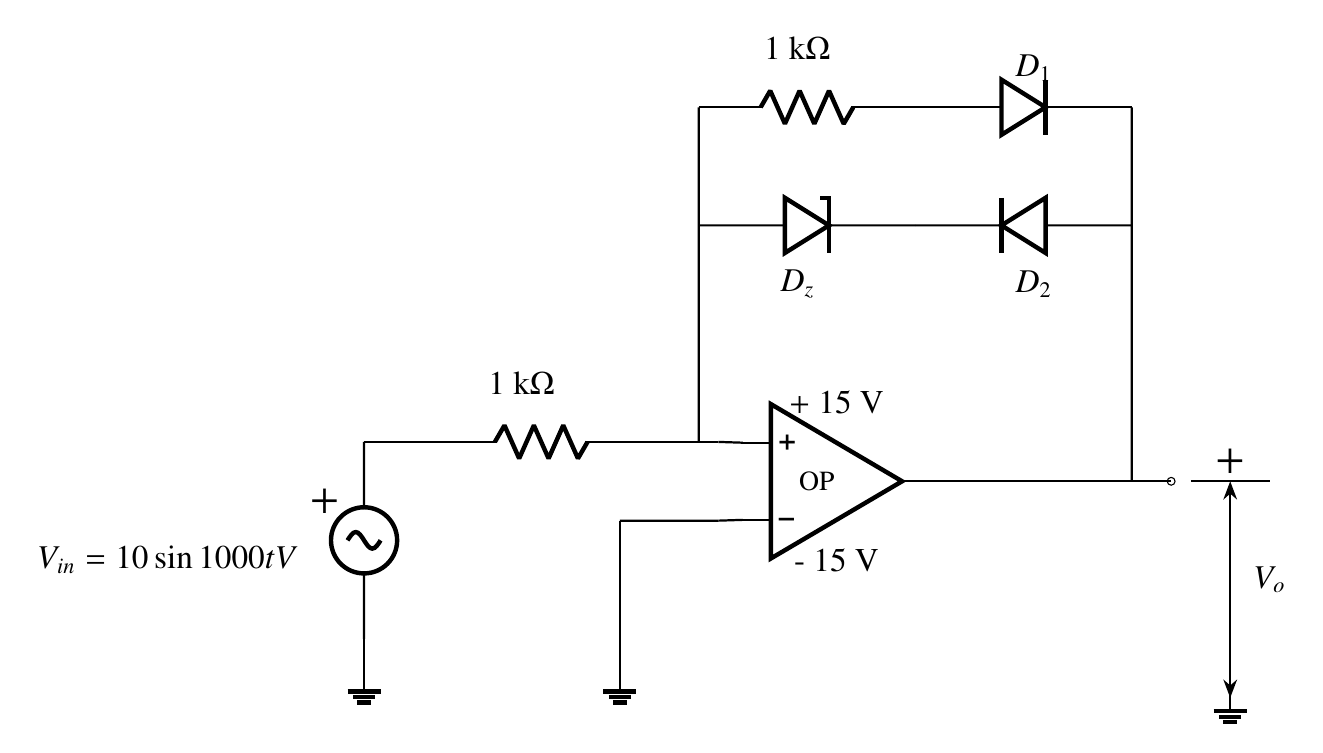
\begin{tikzpicture}[scale = 1]
		\tikzstyle{every node}=[font=\LARGE]
		\draw [line width=0.8pt](8.75,11.25) to[sinusoidal voltage source, sources/symbol/rotate=auto] (8.75,13.75);
		\draw [line width=0.8pt](8.75,13.75) to[R] (13.25,13.75);
		\draw [line width=0.8pt](12,11.25) to[short] (12,12.75);
		\draw [line width=0.8pt](12,12.75) to[short] (13.25,12.75);
		\draw [line width=0.8pt](8.75,11.25) to (8.75,11) node[ground]{};
		\draw [line width=0.8pt](12,11.25) to (12,11) node[ground]{};
		\draw [line width=0.8pt](14.75,13.25) node[op amp, scale=1, yscale=-1] (opamp2) {};
		\draw [line width=0.8pt](opamp2.+) to[short] (13.25,13.75);
		\draw [line width=0.8pt](opamp2.-) to[short] (13.25,12.75);
		\draw [line width=0.8pt](15.95,13.25) to[short] (16.25,13.25);
		\draw [line width=0.8pt](16.25,13.25) to[short] (19,13.25);
		\draw [line width=0.8pt](18.5,13.25) to[short] (18.5,18);
		\draw [line width=0.8pt](13,13.75) to[short] (13,18);
		\draw [line width=0.8pt](13,18) to[R] (15.75,18);
		\draw [line width=0.8pt](15.75,18) to[D] (18.5,18);
		\draw [line width=0.8pt](13,16.5) to[empty Zener diode] (15.75,16.5);
		\draw [line width=0.8pt](18.5,16.5) to[D] (15.75,16.5);
		\node at (19,13.25) [draw, circle, inner sep=1pt] {};
		\draw [line width=0.8pt](19.25,13.25) to[short] (20.25,13.25);
		\draw [line width=0.8pt](19.75,11) to (19.75,10.75) node[ground]{};
		\draw [line width=0.8pt, <->, >=Stealth] (19.75,13.25) -- (19.75,10.5);
		\node [font=\large] at (6.25,12.25) {$V_{in} = 10\sin{1000t} V$};
		\node [font=\large] at (10.75,14.5) {1 k$\Omega$};
		\node [font=\normalsize] at (14.5,13.25) {OP};
		\node [font=\large] at (14.25,18.75) {1 k$\Omega$};
		\node [font=\large] at (17.25,18.5) {$D_1$};
		\node [font=\large] at (17.25,15.75) {$D_2$};
		\node [font=\large] at (14.25,15.75) {$D_z$};
		\node [font=\large] at (14.75,14.25) {+ 15 V};
		\node [font=\large] at (14.75,12.25) {- 15 V};
		\node [font=\large] at (20.25,12) {$V_o$};
		\node [font=\LARGE] at (19.75,13.5) {+};
		\node [font=\LARGE] at (8.25,13) {+};
	\end{tikzpicture}
\end{center}

\begin{enumerate}
	\item The maximum and minimum values of the output voltage $V_O$ are $+15$ V and $-10$ V, respectively.
	\item The maximum and minimum values of the output voltage $V_O$ are $+5$ V and $-15$ V, respectively.
	\item The maximum and minimum values of the output voltage $V_O$ are $+10$ V and $-5$ V, respectively.
	\item The maximum and minimum values of the output voltage $V_O$ are $+5$ V and $-10$ V, respectively.
\end{enumerate}

\item Consider a lead compensator of the form
\[
K(s) = \frac{1 + \frac{s}{a}}{1 + \frac{s}{\beta a}}, \quad \beta > 1, \, a > 0
\]
The frequency at which this compensator produces maximum phase lead is 4 rad/s. At this frequency, the gain amplification provided by the controller, assuming asymptotic Bode-magnitude plot of \( K(s) \), is 6 dB. The values of \( a \) and \( \beta \), respectively, are

\begin{enumerate}
	\item 1, 16
	\item 2, 4
	\item 3, 5
	\item 2.66, 2.25
\end{enumerate}

\item A 3-phase, star-connected, balanced load is supplied from a 3-phase, 400 V (rms), balanced voltage source with phase sequence $R$-$Y$-$B$, as shown in the figure. If the wattmeter reading is $-400$ W and the line current is $I_R = 2$ A (rms), then the power factor of the load per phase is

\begin{center}
	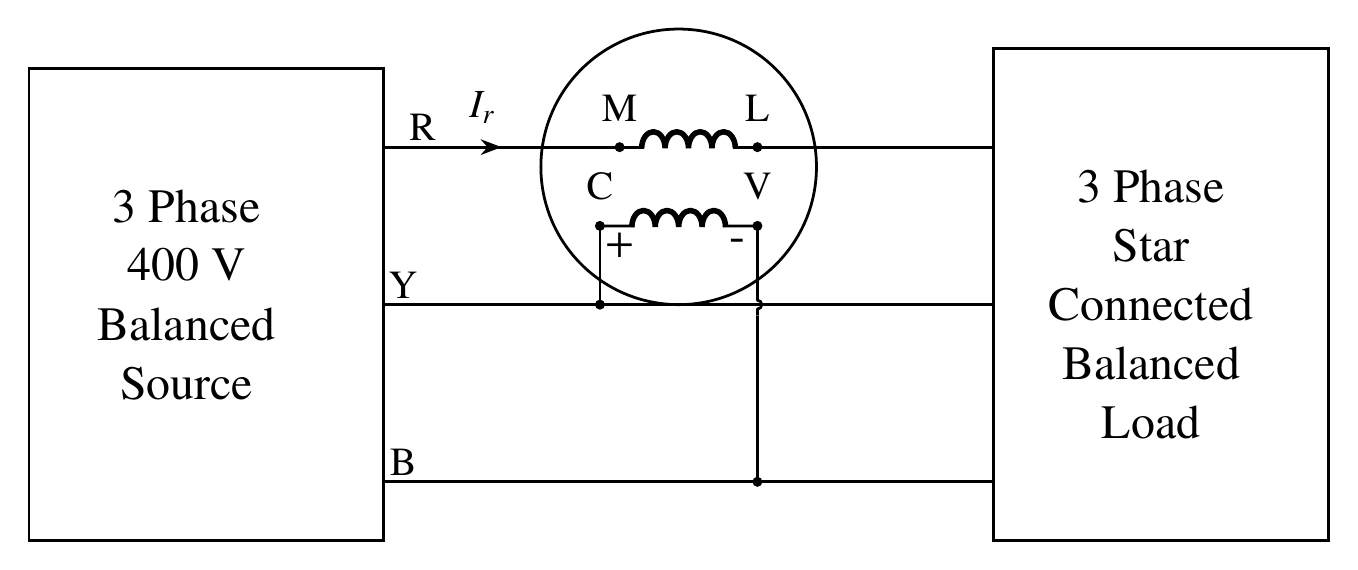
\begin{tikzpicture}[scale = 1]
		\tikzstyle{every node}=[font=\Large]
		\draw [ line width=1pt ] (4.5,14.5) rectangle (9,8.5);
		\draw [ line width=1pt ] (16.75,14.75) rectangle (21,8.5);
		\draw [line width=1pt, short] (9,11.5) -- (16.75,11.5);
		\draw [line width=1pt, short] (9,9.25) -- (16.75,9.25);
		\draw [line width=1pt](9,13.5) to[L ] (16.75,13.5);
		\draw [ line width=1pt](11.75,12.5) to[short] (11.75,11.5);
		\draw [line width=1pt](11.75,12.5) to[L ] (13.75,12.5);
		\draw [ line width=1pt](13.75,12.5) to[short] (13.75,12);
		\draw [ line width=1pt](13.75,11) to[short] (13.75,9.25);
		\draw [ line width=1pt](13.75,12) to[crossing] (13.75,11);
		\node at (12,13.5) [circ] {};
		\node at (13.75,13.5) [circ] {};
		\node at (11.75,12.5) [circ] {};
		\node at (13.75,12.5) [circ] {};
		\node at (11.75,11.5) [circ] {};
		\node at (13.75,9.25) [circ] {};
		\node [font=\LARGE] at (12,12.25) {+};
		\node [font=\LARGE] at (13.5,12.25) {-};
		\draw [line width=1pt, ->, >=Stealth] (9.75,13.5) -- (10.5,13.5);
		\node [font=\LARGE] at (6.5,12.75) {3 Phase};
		\node [font=\LARGE] at (6.5,12) {400 V};
		\node [font=\LARGE] at (6.5,11.25) {Balanced};
		\node [font=\LARGE] at (6.5,10.5) {Source};
		\node [font=\LARGE] at (18.75,13) {3 Phase};
		\node [font=\LARGE] at (18.75,12.25) {Star};
		\node [font=\LARGE] at (18.75,11.5) {Connected};
		\node [font=\LARGE] at (18.75,10.75) {Balanced};
		\node [font=\LARGE] at (18.75,10) {Load};
		\draw [ line width=1pt ] (12.75,13.25) circle (1.75cm);
		\node [font=\Large] at (12,14) {M};
		\node [font=\Large] at (13.75,14) {L};
		\node [font=\Large] at (11.75,13) {C};
		\node [font=\Large] at (13.75,13) {V};
		\node [font=\Large] at (9.5,13.75) {R};
		\node [font=\Large] at (9.25,11.75) {Y};
		\node [font=\Large] at (9.25,9.5) {B};
		\node [font=\Large] at (10.25,14) {$I_r$};
	\end{tikzpicture}
\end{center}

\begin{enumerate}
	\item Unity
	\item $0.5$ leading
	\item $0.866$ leading
	\item $0.707$ lagging
\end{enumerate}


\end{enumerate}
\end{document}


